% Options for packages loaded elsewhere
\PassOptionsToPackage{unicode}{hyperref}
\PassOptionsToPackage{hyphens}{url}
%
\documentclass[
]{article}
\usepackage{lmodern}
\usepackage{amssymb,amsmath}
\usepackage{ifxetex,ifluatex}
\ifnum 0\ifxetex 1\fi\ifluatex 1\fi=0 % if pdftex
  \usepackage[T1]{fontenc}
  \usepackage[utf8]{inputenc}
  \usepackage{textcomp} % provide euro and other symbols
\else % if luatex or xetex
  \usepackage{unicode-math}
  \defaultfontfeatures{Scale=MatchLowercase}
  \defaultfontfeatures[\rmfamily]{Ligatures=TeX,Scale=1}
\fi
% Use upquote if available, for straight quotes in verbatim environments
\IfFileExists{upquote.sty}{\usepackage{upquote}}{}
\IfFileExists{microtype.sty}{% use microtype if available
  \usepackage[]{microtype}
  \UseMicrotypeSet[protrusion]{basicmath} % disable protrusion for tt fonts
}{}
\makeatletter
\@ifundefined{KOMAClassName}{% if non-KOMA class
  \IfFileExists{parskip.sty}{%
    \usepackage{parskip}
  }{% else
    \setlength{\parindent}{0pt}
    \setlength{\parskip}{6pt plus 2pt minus 1pt}}
}{% if KOMA class
  \KOMAoptions{parskip=half}}
\makeatother
\usepackage{xcolor}
\IfFileExists{xurl.sty}{\usepackage{xurl}}{} % add URL line breaks if available
\IfFileExists{bookmark.sty}{\usepackage{bookmark}}{\usepackage{hyperref}}
\hypersetup{
  pdftitle={Decision Trees and Random Forest classifiers},
  pdfauthor={R Mofidi},
  hidelinks,
  pdfcreator={LaTeX via pandoc}}
\urlstyle{same} % disable monospaced font for URLs
\usepackage[margin=1in]{geometry}
\usepackage{color}
\usepackage{fancyvrb}
\newcommand{\VerbBar}{|}
\newcommand{\VERB}{\Verb[commandchars=\\\{\}]}
\DefineVerbatimEnvironment{Highlighting}{Verbatim}{commandchars=\\\{\}}
% Add ',fontsize=\small' for more characters per line
\usepackage{framed}
\definecolor{shadecolor}{RGB}{248,248,248}
\newenvironment{Shaded}{\begin{snugshade}}{\end{snugshade}}
\newcommand{\AlertTok}[1]{\textcolor[rgb]{0.94,0.16,0.16}{#1}}
\newcommand{\AnnotationTok}[1]{\textcolor[rgb]{0.56,0.35,0.01}{\textbf{\textit{#1}}}}
\newcommand{\AttributeTok}[1]{\textcolor[rgb]{0.77,0.63,0.00}{#1}}
\newcommand{\BaseNTok}[1]{\textcolor[rgb]{0.00,0.00,0.81}{#1}}
\newcommand{\BuiltInTok}[1]{#1}
\newcommand{\CharTok}[1]{\textcolor[rgb]{0.31,0.60,0.02}{#1}}
\newcommand{\CommentTok}[1]{\textcolor[rgb]{0.56,0.35,0.01}{\textit{#1}}}
\newcommand{\CommentVarTok}[1]{\textcolor[rgb]{0.56,0.35,0.01}{\textbf{\textit{#1}}}}
\newcommand{\ConstantTok}[1]{\textcolor[rgb]{0.00,0.00,0.00}{#1}}
\newcommand{\ControlFlowTok}[1]{\textcolor[rgb]{0.13,0.29,0.53}{\textbf{#1}}}
\newcommand{\DataTypeTok}[1]{\textcolor[rgb]{0.13,0.29,0.53}{#1}}
\newcommand{\DecValTok}[1]{\textcolor[rgb]{0.00,0.00,0.81}{#1}}
\newcommand{\DocumentationTok}[1]{\textcolor[rgb]{0.56,0.35,0.01}{\textbf{\textit{#1}}}}
\newcommand{\ErrorTok}[1]{\textcolor[rgb]{0.64,0.00,0.00}{\textbf{#1}}}
\newcommand{\ExtensionTok}[1]{#1}
\newcommand{\FloatTok}[1]{\textcolor[rgb]{0.00,0.00,0.81}{#1}}
\newcommand{\FunctionTok}[1]{\textcolor[rgb]{0.00,0.00,0.00}{#1}}
\newcommand{\ImportTok}[1]{#1}
\newcommand{\InformationTok}[1]{\textcolor[rgb]{0.56,0.35,0.01}{\textbf{\textit{#1}}}}
\newcommand{\KeywordTok}[1]{\textcolor[rgb]{0.13,0.29,0.53}{\textbf{#1}}}
\newcommand{\NormalTok}[1]{#1}
\newcommand{\OperatorTok}[1]{\textcolor[rgb]{0.81,0.36,0.00}{\textbf{#1}}}
\newcommand{\OtherTok}[1]{\textcolor[rgb]{0.56,0.35,0.01}{#1}}
\newcommand{\PreprocessorTok}[1]{\textcolor[rgb]{0.56,0.35,0.01}{\textit{#1}}}
\newcommand{\RegionMarkerTok}[1]{#1}
\newcommand{\SpecialCharTok}[1]{\textcolor[rgb]{0.00,0.00,0.00}{#1}}
\newcommand{\SpecialStringTok}[1]{\textcolor[rgb]{0.31,0.60,0.02}{#1}}
\newcommand{\StringTok}[1]{\textcolor[rgb]{0.31,0.60,0.02}{#1}}
\newcommand{\VariableTok}[1]{\textcolor[rgb]{0.00,0.00,0.00}{#1}}
\newcommand{\VerbatimStringTok}[1]{\textcolor[rgb]{0.31,0.60,0.02}{#1}}
\newcommand{\WarningTok}[1]{\textcolor[rgb]{0.56,0.35,0.01}{\textbf{\textit{#1}}}}
\usepackage{graphicx,grffile}
\makeatletter
\def\maxwidth{\ifdim\Gin@nat@width>\linewidth\linewidth\else\Gin@nat@width\fi}
\def\maxheight{\ifdim\Gin@nat@height>\textheight\textheight\else\Gin@nat@height\fi}
\makeatother
% Scale images if necessary, so that they will not overflow the page
% margins by default, and it is still possible to overwrite the defaults
% using explicit options in \includegraphics[width, height, ...]{}
\setkeys{Gin}{width=\maxwidth,height=\maxheight,keepaspectratio}
% Set default figure placement to htbp
\makeatletter
\def\fps@figure{htbp}
\makeatother
\setlength{\emergencystretch}{3em} % prevent overfull lines
\providecommand{\tightlist}{%
  \setlength{\itemsep}{0pt}\setlength{\parskip}{0pt}}
\setcounter{secnumdepth}{-\maxdimen} % remove section numbering

\title{Decision Trees and Random Forest classifiers}
\author{R Mofidi}
\date{24/06/2020}

\begin{document}
\maketitle

\hypertarget{decision-tree-analysis}{%
\subsection{Decision tree Analysis}\label{decision-tree-analysis}}

Decision Trees are a class of tree like graph algorithms. In addition to
being a predictive model decision trees use this tree like structure to
illustrate the possible decisions and their consequences. It is one way
of combining an algorithm and a decision support tool as well as a
machine learning paradigm. A decision tree consists of 3 constituents
(no pun intended), a node which represents an attribute and a branch
which represents the consequences of classifying the dataset based on
that attribute. Attributes can occur as a result of an active decision
(a decision node, usually marked as a square), a chance node which is
the consequences of an event outside of the decision makers' control and
an end node (leaf) which denotes one of the possible final outcomes of
the decision tree algorithm. In this way, the findings of the decision
tree can be illustrated in a compact and easy to follow format using an
influence diagram which describes the relationship between actions and
consequences.

In this way decision tree classifiers utilise the topography of a
decision tree to map observations about a target item to conclusions
about the value of the target item. Where the target value has a finite
set of values (ordinal or nominal), the process is known as a
classification tree. If the Target value is a continuous variable the
resultant model is called regression tree. The umbrella term
Classification and Regression Tree (CART) is used to group both
processes. This class of classifiers were devised by the distinguished
American statistician Leo Breiman who was also involved in their
eventual evolution into random forest classifiers. The CARTs work from
top down by choosing the variables which best splits a set of items into
the intended classes.This is performed by calculating the Gini
coefficient for the putative input variables. The Gini coefficient
denotes the descrminant ability of a variable in correctly classifying
the data according to the output variable (which we are trying to
predict). It is named after the Italian economist, sociologist and
statistician Corrado Gini. The algorithms created are simple to
understand and require little preparation, It is possible to use
categorical as well as continuous variables and create a white box model
which is transparent to the user. It is possible to validate using
statistical models such as a confusion matrix or receiver operator
characteristic test.

Decision tree analysis involves a series of simple steps the first of
which involves identifying and using the variable which best separates
the dataset in accordance with the outcome of interest. This creates 2
leaves or childeren nodes. the remaining data set in each leaves is
divided in a similar manner until the groups are either too small or
pure i.e.~contain only a single outcome (pure). Some software programs
create competing Trees and eliminate the ones which have lower
predictive ability based on in sample testing.

\hypertarget{the-fishers-or-andersons-iris-dataset}{%
\subsubsection{The Fisher's or Anderson's iris
dataset}\label{the-fishers-or-andersons-iris-dataset}}

The following example is created using a commonly encountered database
in R known as the Iris database. This databse uses the width and length
of the petal and sepal of iris floweres to classify the iris flowers
into the 3 different species: 1- Setosa 2- Versicolor 3- Virginica

The follollowing code describes how decision trees (classification and
Regression Trees) can be developed in R.

\hypertarget{install-the-appropriate-libraries-and-datasets}{%
\subsection{Install the appropriate libraries and
datasets}\label{install-the-appropriate-libraries-and-datasets}}

Clearly the first step in R involves downloading the appropriate
packages required:

\begin{Shaded}
\begin{Highlighting}[]
\KeywordTok{data}\NormalTok{(iris)}
\KeywordTok{library}\NormalTok{(caret)}
\end{Highlighting}
\end{Shaded}

\begin{verbatim}
## Loading required package: lattice
\end{verbatim}

\begin{verbatim}
## Loading required package: ggplot2
\end{verbatim}

\begin{Shaded}
\begin{Highlighting}[]
\KeywordTok{library}\NormalTok{(ggplot2)}
\KeywordTok{library}\NormalTok{(lattice)}
\KeywordTok{head}\NormalTok{(iris)}
\end{Highlighting}
\end{Shaded}

\begin{verbatim}
##   Sepal.Length Sepal.Width Petal.Length Petal.Width Species
## 1          5.1         3.5          1.4         0.2  setosa
## 2          4.9         3.0          1.4         0.2  setosa
## 3          4.7         3.2          1.3         0.2  setosa
## 4          4.6         3.1          1.5         0.2  setosa
## 5          5.0         3.6          1.4         0.2  setosa
## 6          5.4         3.9          1.7         0.4  setosa
\end{verbatim}

\hypertarget{separate-training-and-test-datasets}{%
\subsubsection{Separate training and test
datasets}\label{separate-training-and-test-datasets}}

The next step involves partitioning the dataset into training and test
datasets. This creates a training dataset for developing the tree and a
testing dataset for cross validation:

\begin{Shaded}
\begin{Highlighting}[]
\NormalTok{inTrain3<-}\StringTok{ }\KeywordTok{createDataPartition}\NormalTok{(}\DataTypeTok{y=}\NormalTok{iris}\OperatorTok{$}\NormalTok{Species, }\DataTypeTok{p=}\FloatTok{0.7}\NormalTok{, }\DataTypeTok{list=}\OtherTok{FALSE}\NormalTok{)}
\NormalTok{trainingDS<-}\StringTok{ }\NormalTok{iris[inTrain3,]}
\NormalTok{testingDS<-}\StringTok{ }\NormalTok{iris[}\OperatorTok{-}\NormalTok{inTrain3,]}
\KeywordTok{dim}\NormalTok{ (trainingDS); }\KeywordTok{dim}\NormalTok{(testingDS)}
\end{Highlighting}
\end{Shaded}

\begin{verbatim}
## [1] 105   5
\end{verbatim}

\begin{verbatim}
## [1] 45  5
\end{verbatim}

\hypertarget{make-a-plot-to-view-data-separation}{%
\section{Make a plot to view data
separation}\label{make-a-plot-to-view-data-separation}}

It is very useful to see the separation between the data clusters

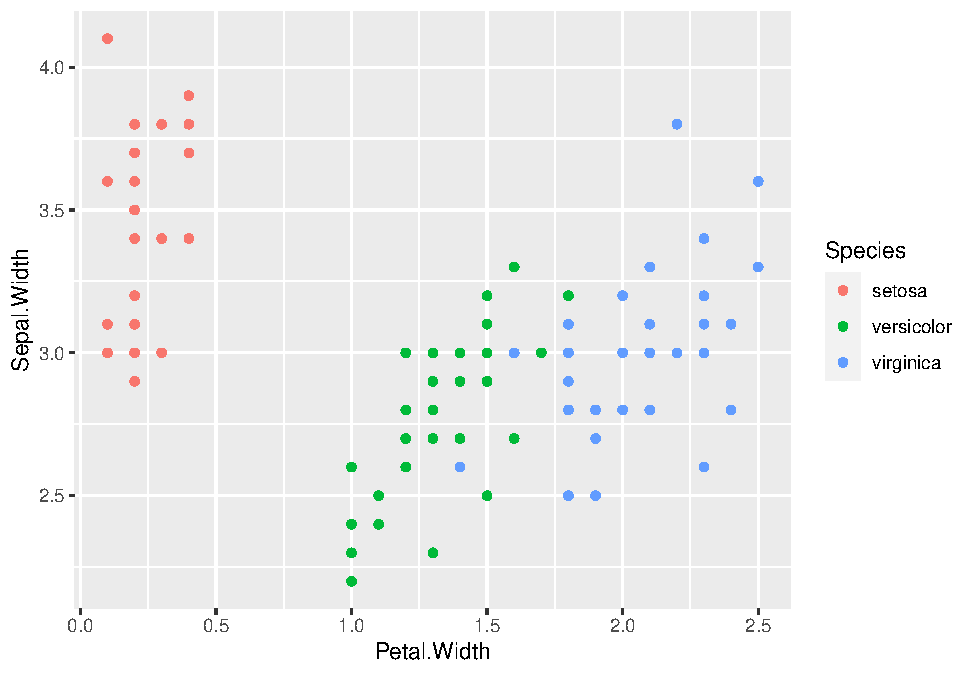
\includegraphics{crtrf_files/figure-latex/unnamed-chunk-3-1.pdf}

\hypertarget{developing-the-decision-tree-rpart-model.}{%
\section{developing the decision tree ``rpart''
model.}\label{developing-the-decision-tree-rpart-model.}}

\begin{Shaded}
\begin{Highlighting}[]
\KeywordTok{library}\NormalTok{(caret)}
\NormalTok{modfit<-}\StringTok{ }\KeywordTok{train}\NormalTok{(Species}\OperatorTok{~}\NormalTok{.,}\DataTypeTok{method=}\StringTok{"rpart"}\NormalTok{, }\DataTypeTok{data=}\NormalTok{trainingDS)}
\KeywordTok{print}\NormalTok{(modfit}\OperatorTok{$}\NormalTok{finalModel)}
\end{Highlighting}
\end{Shaded}

\begin{verbatim}
## n= 105 
## 
## node), split, n, loss, yval, (yprob)
##       * denotes terminal node
## 
## 1) root 105 70 setosa (0.33333333 0.33333333 0.33333333)  
##   2) Petal.Length< 2.6 35  0 setosa (1.00000000 0.00000000 0.00000000) *
##   3) Petal.Length>=2.6 70 35 versicolor (0.00000000 0.50000000 0.50000000)  
##     6) Petal.Length< 4.85 34  2 versicolor (0.00000000 0.94117647 0.05882353) *
##     7) Petal.Length>=4.85 36  3 virginica (0.00000000 0.08333333 0.91666667) *
\end{verbatim}

\#\#Plot modelfit classification Tree

\begin{verbatim}
## Loading required package: tibble
\end{verbatim}

\begin{verbatim}
## Loading required package: bitops
\end{verbatim}

\begin{verbatim}
## Rattle: A free graphical interface for data science with R.
## Version 5.4.0 Copyright (c) 2006-2020 Togaware Pty Ltd.
## Type 'rattle()' to shake, rattle, and roll your data.
\end{verbatim}

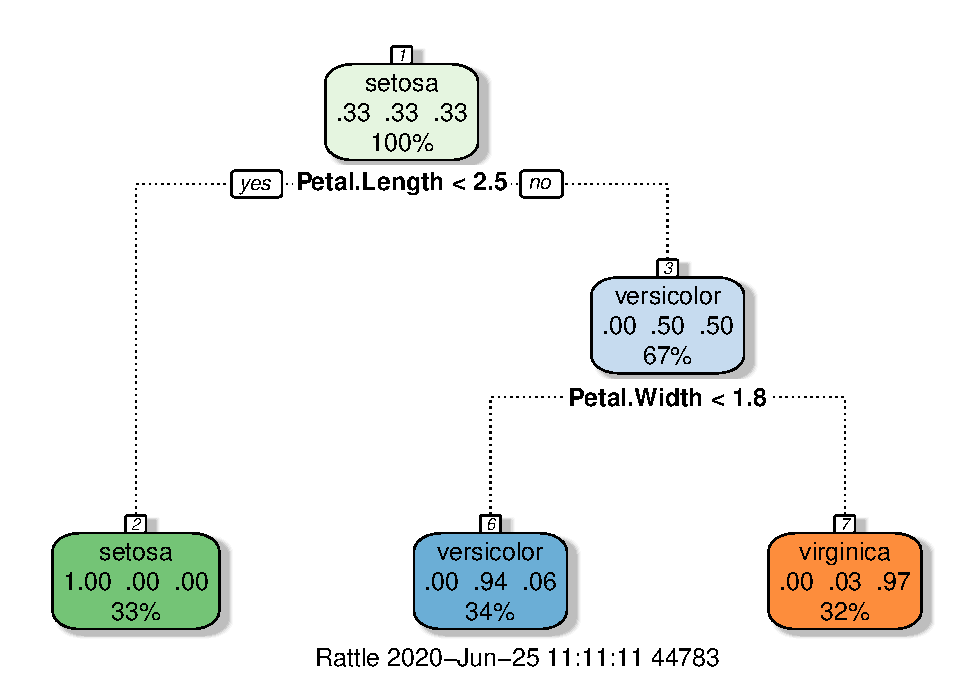
\includegraphics{crtrf_files/figure-latex/unnamed-chunk-5-1.pdf}

\hypertarget{crossvalidation-using-perofrming-the-prediction-on-the-testing-sample}{%
\section{Crossvalidation using perofrming the prediction on the testing
sample:}\label{crossvalidation-using-perofrming-the-prediction-on-the-testing-sample}}

\begin{Shaded}
\begin{Highlighting}[]
\KeywordTok{predict}\NormalTok{(modfit, }\DataTypeTok{newdata=}\NormalTok{testingDS)}
\end{Highlighting}
\end{Shaded}

\begin{verbatim}
##  [1] setosa     setosa     setosa     setosa     setosa     setosa    
##  [7] setosa     setosa     setosa     setosa     setosa     setosa    
## [13] setosa     setosa     setosa     versicolor virginica  versicolor
## [19] versicolor versicolor versicolor versicolor versicolor versicolor
## [25] versicolor versicolor versicolor versicolor versicolor versicolor
## [31] virginica  virginica  virginica  virginica  virginica  virginica 
## [37] virginica  virginica  virginica  virginica  virginica  versicolor
## [43] virginica  virginica  virginica 
## Levels: setosa versicolor virginica
\end{verbatim}

\begin{Shaded}
\begin{Highlighting}[]
\NormalTok{PredR<-}\StringTok{ }\KeywordTok{predict}\NormalTok{(modfit, }\DataTypeTok{newdata=}\NormalTok{testingDS)}
\KeywordTok{summary}\NormalTok{(PredR)}
\end{Highlighting}
\end{Shaded}

\begin{verbatim}
##     setosa versicolor  virginica 
##         15         15         15
\end{verbatim}

\begin{Shaded}
\begin{Highlighting}[]
\KeywordTok{qplot}\NormalTok{(Petal.Width, Petal.Length, }\DataTypeTok{colour=}\NormalTok{PredR,}\DataTypeTok{data=}\NormalTok{testingDS, }\DataTypeTok{main =} \StringTok{"out of sample accuracy"}\NormalTok{)}
\end{Highlighting}
\end{Shaded}

\includegraphics{crtrf_files/figure-latex/unnamed-chunk-6-1.pdf}

\#\#Random Forests and Ensamble Classifiers

Ensemble Classifiers a consist of multiple classifiers which by
themselves may be weak (i.e.~have low predictive ability) but combining
them into an ensemble improves their predictive ability significantly. A
similar concept exists in statistics with the difference that machine
learning the ensembles contain a finite set of constituent algorithms
whilst a statistical ensemble is infinite. The design of this class of
algorithm is based on ensemble theory which states that a trained
ensemble of algorithms can represent a single supervised trained
algorithm. In general an ensemble algorithm functions better if it
contains a diverse set of constituent algorithms.

In fact the individual constituents of the ensemble do not necessarily
have to be weak classifiers, being part of the ensemble means that they
do not need to be complex in structure which in turn helps protect
against over-fitting (over-training). They key to a successful ensemble
is ``stochastic discrimination'' which is discussed later. There are a
number of classes of ensemble classifiers in existence they include: •
Bayes optimal classifiers • Bootstrap aggregating methods such as Random
forest classifiers • Boosting: such as Adaboost

In this paper we discuss random forest classfiers

\hypertarget{random-forest-classifiers}{%
\subsubsection{Random Forest
classifiers}\label{random-forest-classifiers}}

An example of ensemble classifiers is the random forest. Random forests
were first designed by the American data scientist Tin Kam Ho in the
1990s. Random forests are made up of (large) number of tree classifiers
which are added together in an ensemble in order to improve their
classification ability. It is a bootstrap aggregating method which means
each of these decision tree classifiers contributes to the eventual
decision with an equal weight.

Each tree acts as a weak classifier and together a large number of trees
form a random forest and diversity of classifiers within the ensemble is
the key to its performance.

If you remember in order to develop an ensemble classifier two
assumptions will need to be fulfilled. The 2nd of these two assumptions
is that each weak classifier should make its choice independently of the
other classifiers. This concept is called ``Stochastic discrimination''.
In order to fulfil this assumption each decision tree needs to undergo a
different training process using the same training data. This is a
dilemma as often the training data is scarce. One way of getting around
this is randomisation (random selection) of training data he used to
train each tree classifier. In order to develop a random forest during
training process a number of hyperplanes are selected at random and are
trained using a random sub set of they are available training data. The
final classification is performed using a majority vote

The following is an example of a small random forest classifier created
using the iris database described above:

\#\#\#loading the required packages and database

\begin{Shaded}
\begin{Highlighting}[]
\KeywordTok{data}\NormalTok{(iris); }\KeywordTok{library}\NormalTok{(ggplot2); }\KeywordTok{library}\NormalTok{(randomForest);}\KeywordTok{library}\NormalTok{(caret)}
\end{Highlighting}
\end{Shaded}

\begin{verbatim}
## randomForest 4.6-14
\end{verbatim}

\begin{verbatim}
## Type rfNews() to see new features/changes/bug fixes.
\end{verbatim}

\begin{verbatim}
## 
## Attaching package: 'randomForest'
\end{verbatim}

\begin{verbatim}
## The following object is masked from 'package:rattle':
## 
##     importance
\end{verbatim}

\begin{verbatim}
## The following object is masked from 'package:ggplot2':
## 
##     margin
\end{verbatim}

\#\#\#partitioning the data into training and testing sets

\begin{Shaded}
\begin{Highlighting}[]
\NormalTok{inTrainRF<-}\KeywordTok{createDataPartition}\NormalTok{(}\DataTypeTok{y=}\NormalTok{iris}\OperatorTok{$}\NormalTok{Species, }\DataTypeTok{p=}\FloatTok{0.7}\NormalTok{, }\DataTypeTok{list=}\OtherTok{FALSE}\NormalTok{)}
\NormalTok{training4<-iris[inTrainRF,]}
\NormalTok{testing4<-iris[}\OperatorTok{-}\NormalTok{inTrainRF,]}
\end{Highlighting}
\end{Shaded}

\hypertarget{training-the-random-forest-classifier}{%
\subsubsection{Training the random forest
classifier:}\label{training-the-random-forest-classifier}}

This involves setting the output variable as the Species and the rest of
the variables as input variables.

\begin{Shaded}
\begin{Highlighting}[]
\NormalTok{modFit<-}\StringTok{ }\KeywordTok{train}\NormalTok{(Species}\OperatorTok{~}\NormalTok{.,}\DataTypeTok{data=}\NormalTok{training4, }\DataTypeTok{method=}\StringTok{"rf"}\NormalTok{, }\DataTypeTok{prox=}\OtherTok{TRUE}\NormalTok{)}
\NormalTok{modFit}
\end{Highlighting}
\end{Shaded}

\begin{verbatim}
## Random Forest 
## 
## 105 samples
##   4 predictor
##   3 classes: 'setosa', 'versicolor', 'virginica' 
## 
## No pre-processing
## Resampling: Bootstrapped (25 reps) 
## Summary of sample sizes: 105, 105, 105, 105, 105, 105, ... 
## Resampling results across tuning parameters:
## 
##   mtry  Accuracy   Kappa    
##   2     0.9497409  0.9230556
##   3     0.9497409  0.9230556
##   4     0.9486113  0.9214384
## 
## Accuracy was used to select the optimal model using the largest value.
## The final value used for the model was mtry = 2.
\end{verbatim}

As you can see the in sample accuracy od the data is excellent and it
overperforms most linear data models as well as Classification and
regression trees. clearly concerns regarding over-training (overfitting
the data exists. This is why cross validation and data visualization is
important. This is what the testing sample ``testing4'' is used for.
Random forests can be complicated in order to understand their
underlying anatomy, it is possible to view the consituent trees making
up the random forest classifier:

\begin{Shaded}
\begin{Highlighting}[]
\KeywordTok{getTree}\NormalTok{(modFit}\OperatorTok{$}\NormalTok{finalModel,}\DataTypeTok{k=}\DecValTok{2}\NormalTok{)}
\end{Highlighting}
\end{Shaded}

\begin{verbatim}
##    left daughter right daughter split var split point status prediction
## 1              2              3         4        0.80      1          0
## 2              0              0         0        0.00     -1          1
## 3              4              5         3        4.85      1          0
## 4              6              7         3        4.75      1          0
## 5              8              9         1        6.85      1          0
## 6              0              0         0        0.00     -1          2
## 7             10             11         4        1.60      1          0
## 8              0              0         0        0.00     -1          3
## 9             12             13         1        7.05      1          0
## 10             0              0         0        0.00     -1          2
## 11            14             15         1        5.95      1          0
## 12             0              0         0        0.00     -1          2
## 13             0              0         0        0.00     -1          3
## 14             0              0         0        0.00     -1          2
## 15             0              0         0        0.00     -1          3
\end{verbatim}

\hypertarget{visualising-the-classifier}{%
\paragraph{Visualising the
classifier}\label{visualising-the-classifier}}

\begin{Shaded}
\begin{Highlighting}[]
\NormalTok{irisP<-}\StringTok{ }\KeywordTok{classCenter}\NormalTok{(training4[,}\KeywordTok{c}\NormalTok{(}\DecValTok{3}\NormalTok{,}\DecValTok{4}\NormalTok{)], training4}\OperatorTok{$}\NormalTok{Species, modFit}\OperatorTok{$}\NormalTok{finalModel}\OperatorTok{$}\NormalTok{prox)}
\NormalTok{irisP<-}\KeywordTok{as.data.frame}\NormalTok{(irisP);irisP}\OperatorTok{$}\NormalTok{Species<-}\StringTok{ }\KeywordTok{rownames}\NormalTok{(irisP)}
\NormalTok{P<-}\StringTok{ }\KeywordTok{qplot}\NormalTok{(Petal.Width, Petal.Length, }\DataTypeTok{col=}\NormalTok{Species, }\DataTypeTok{size=}\DecValTok{2}\NormalTok{,}\DataTypeTok{Shape=}\DecValTok{4}\NormalTok{,}\DataTypeTok{data=}\NormalTok{training4)}
\end{Highlighting}
\end{Shaded}

\begin{verbatim}
## Warning: Ignoring unknown parameters: Shape
\end{verbatim}

\begin{Shaded}
\begin{Highlighting}[]
\NormalTok{P}\OperatorTok{+}\KeywordTok{geom_point}\NormalTok{(}\KeywordTok{aes}\NormalTok{(}\DataTypeTok{x=}\NormalTok{Petal.Width, }\DataTypeTok{y=}\NormalTok{Petal.Length, }\DataTypeTok{col=}\NormalTok{Species), }\DataTypeTok{size=}\DecValTok{2}\NormalTok{, }\DataTypeTok{shape=}\DecValTok{4}\NormalTok{, }\DataTypeTok{data=}\NormalTok{irisP)}
\end{Highlighting}
\end{Shaded}

\includegraphics{crtrf_files/figure-latex/unnamed-chunk-11-1.pdf}

\hypertarget{making-the-prediction-in-the-testing-sample}{%
\subsubsection{Making the prediction in the testing
sample}\label{making-the-prediction-in-the-testing-sample}}

This is the process of cross validation of the classifier.

\begin{Shaded}
\begin{Highlighting}[]
\NormalTok{pred<-}\KeywordTok{predict}\NormalTok{(modFit, testing4) }
\NormalTok{testing4}\OperatorTok{$}\NormalTok{predRight<-pred }\OperatorTok{==}\StringTok{ }\NormalTok{testing4}\OperatorTok{$}\NormalTok{Species}
\KeywordTok{table}\NormalTok{(pred,testing4}\OperatorTok{$}\NormalTok{Species)}
\end{Highlighting}
\end{Shaded}

\begin{verbatim}
##             
## pred         setosa versicolor virginica
##   setosa         15          0         0
##   versicolor      0         14         2
##   virginica       0          1        13
\end{verbatim}

\includegraphics{crtrf_files/figure-latex/unnamed-chunk-13-1.pdf}

Random forests are amongst the most powerful classifiers available and
as you can see at a very basic level they are not too difficult to
develop in R. Despite their complexity which can be a problem when
dealing with large data sets, they are considered white-box classifiers.
Well implemented random forests are more resiliant to overfitting Random
forests have less variance than single decision trees.

Complexity when large ensambles are being used to analyse large
datasets. This can be time consuming and complicated process.

\end{document}
